\documentclass[a4paper,11pt]{article}
\usepackage{sbpo-template}
%\usepackage[latin1]{inputenc}
\usepackage[brazil]{babel}    % português do Brasil
\usepackage[utf8]{inputenc}   % acentos no UTF-8
\usepackage[T1]{fontenc}      % para hifenização correta
\usepackage{amsmath,amssymb}
\usepackage{url}
\usepackage[square]{natbib}
\usepackage{indentfirst}
\usepackage{fancyhdr}
\usepackage{graphicx}
\pagestyle{fancy}
\fancyhf{}
\fancyhead[C]{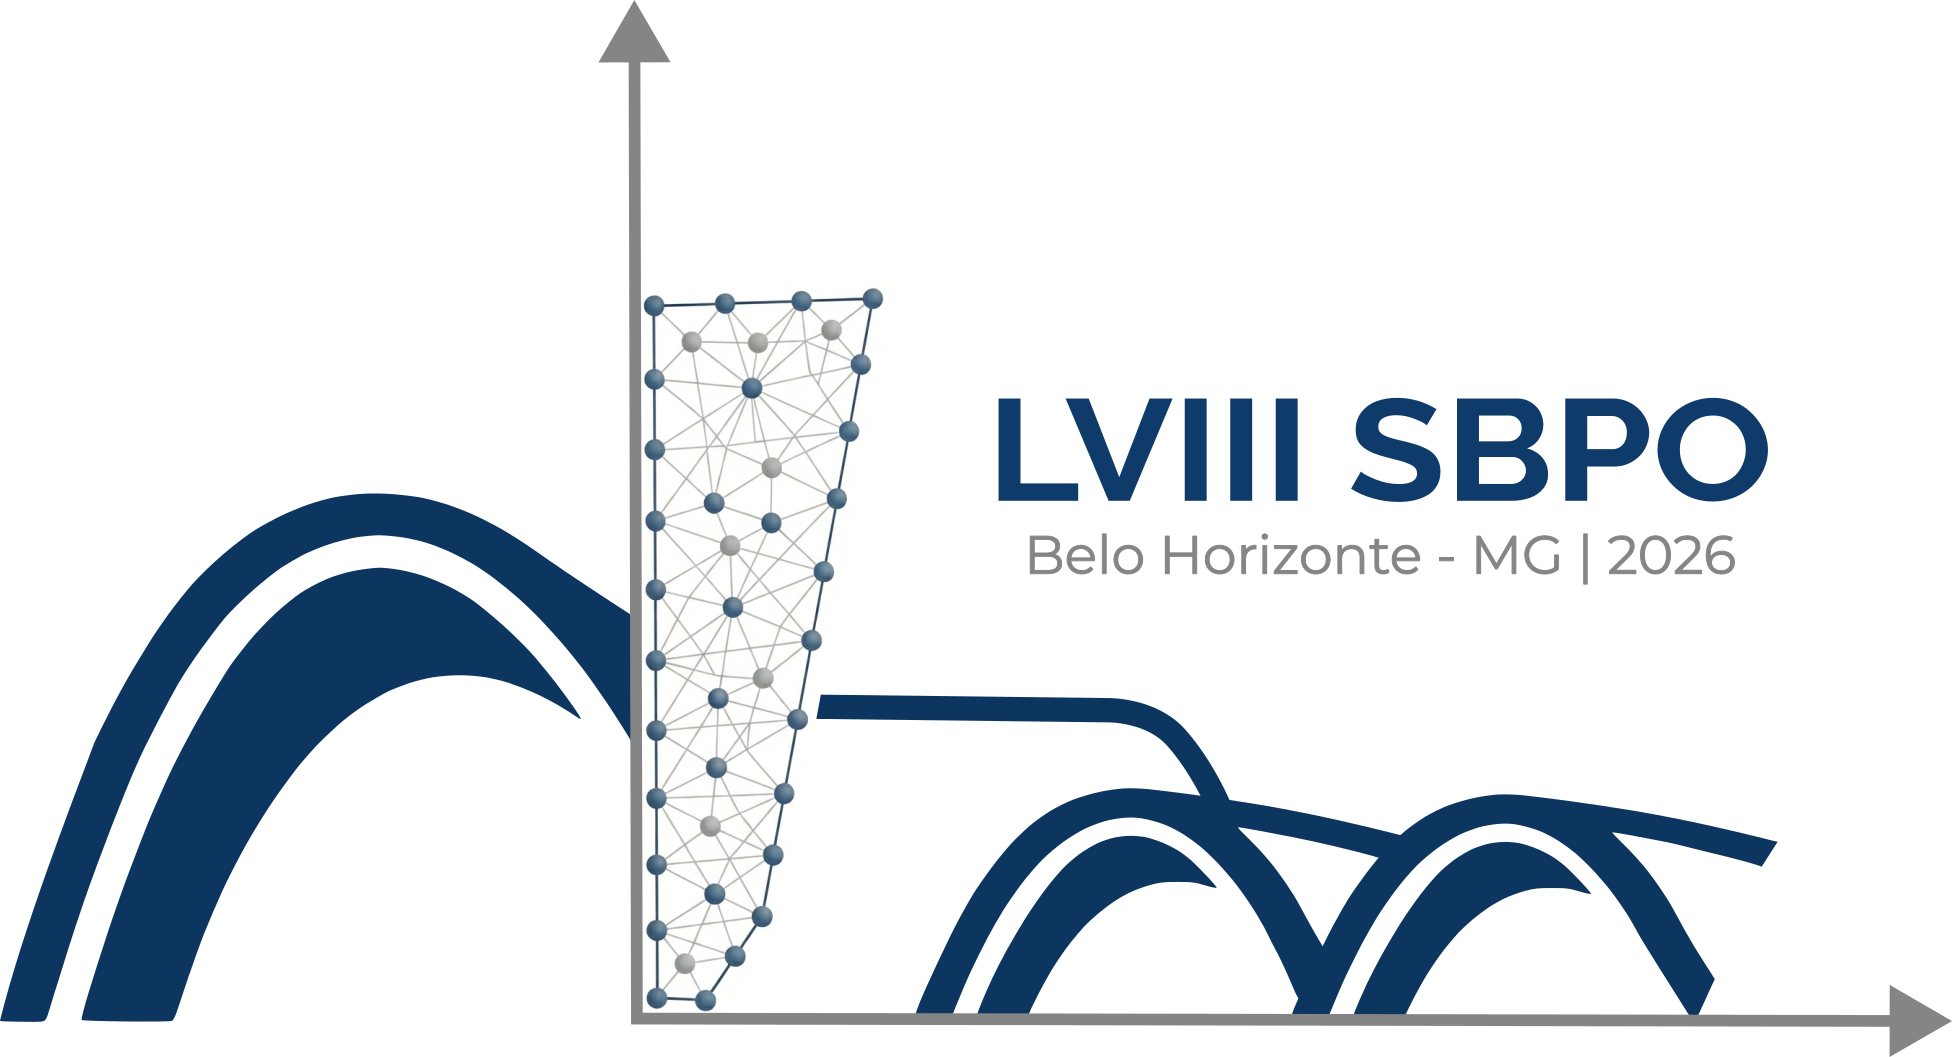
\includegraphics[scale=0.5]{sbpo2026-header-logo.png}}
%\renewcommand{\headrulewidth}{0pt}
\renewcommand{\headruleskip}{-1mm}
%\setlength\headheight{101.0pt}
%\addtolength{\textheight}{-101.0pt}
\setlength\headheight{86pt}
\addtolength{\textheight}{-86pt}
\setlength{\headsep}{5mm}
\setlength{\footskip}{4.08003pt}

\begin{document}

\title{GESTÃO DINÂMICA DE PORTFÓLIO DE CONTRATOS DE ENERGIA: \\ COMPARAÇÃO ENTRE EQUIVALENTE DETERMINÍSTICO E SDDP} 

\maketitle
\thispagestyle{fancy}

\author{
\name{Lucas Garcia}
\institute{Universidade Federal do Rio de Janeiro (UFRJ)}
\iaddress{Rio de Janeiro - RJ}
\email{lucas.garcia@ufrj.br}
}

\author{ 
\name{Nome do Orientador}
\institute{Universidade Federal do Rio de Janeiro (UFRJ)} 
\iaddress{Rio de Janeiro - RJ}
\email{orientador@ufrj.br}
}

\author{ 
\name{Nome do Orientador}
\institute{Universidade Federal do Rio de Janeiro (UFRJ)} 
\iaddress{Rio de Janeiro - RJ}
\email{orientador@ufrj.br}
}

\vspace{8mm}
\begin{resumo}
Este trabalho aborda o problema de gestão de portfólio de uma comercializadora de energia elétrica exposta ao Preço de Liquidação de Diferenças (PLD). Propõe-se uma modelagem estocástica multiestágio para otimizar decisões de compra e venda de contratos bilaterais sob incerteza climática e de preços. Comparam-se duas abordagens clássicas: o Equivalente Determinístico (DEQ), via árvore de cenários, e a Programação Dinâmica Dual Estocástica (SDDP). Os resultados demonstram que, embora ambos convirjam para a política ótima em instâncias de menor dimensão, o DEQ apresenta um estrangulamento crítico de memória RAM devido ao overhead algébrico na formulação da matriz, enquanto o SDDP mantém a tratabilidade computacional para horizontes expandidos.
\end{resumo}

\bigskip
\begin{palchaves}
Otimização Estocástica, SDDP, Mercado de Energia, JuMP.

\bigskip
\noindent{Tópicos (indique, em ordem de PRIORIDADE, o(s) tópicos(s) de seu artigo) }
\end{palchaves}

\vspace{8mm}

\begin{abstract}
This paper addresses the portfolio management problem for an energy trading company exposed to the Settlement Price for Differences (PLD). A multistage stochastic modeling is proposed to optimize buying and selling decisions of bilateral contracts under climate and price uncertainty. Two classical approaches are compared: the Deterministic Equivalent (DEQ), via scenario trees, and the Stochastic Dual Dynamic Programming (SDDP). Results demonstrate that while both converge to the optimal policy in small instances, DEQ presents a critical RAM bottleneck due to algebraic overhead in matrix formulation, whereas SDDP maintains computational tractability for expanded horizons.
\end{abstract}

\bigskip
\begin{keywords}
Stochastic Optimization, SDDP, Energy Market, JuMP.

\bigskip
\noindent{Paper topics (indicate in order of PRIORITY the paper topic(s))}
\end{keywords}

\newpage
\section{Introdução}
A comercialização de energia no Ambiente de Contratação Livre (ACL) brasileiro exige a tomada de decisões vinculativas antes da revelação da hidrologia e do PLD. Este trabalho foca na gestão de risco de caixa e manutenção de margens de crédito através de modelos multiestágio, comparando os limites computacionais do método de árvore de cenários com o método de decomposição de Benders (SDDP).

% --- ARQUIVO: modelagem-matematica.tex ---
% Este arquivo deve ser incluído no main usando % --- ARQUIVO: modelagem-matematica.tex ---
% Este arquivo deve ser incluído no main usando % --- ARQUIVO: modelagem-matematica.tex ---
% Este arquivo deve ser incluído no main usando \input{modelagem-matematica.tex}

\section{Modelagem Matemática}
\label{sec:modelagem}

Para a implementação da gestão de portfólio de contratos, propõe-se inicialmente a formulação do Equivalente Determinístico (DEQ) em formato de árvore de cenários. As variáveis e restrições são indexadas por nós da árvore, preservando a dependência intertemporal e a não-antecipatividade inerentes ao mercado de energia.

\subsection{Notação: Conjuntos, Parâmetros e Variáveis}

Seja $\mathcal{N}$ o conjunto de nós da árvore de cenários, onde $a(n)$ denota o nó pai do nó $n$, e $\mathcal{L} \subset \mathcal{N}$ o subconjunto de nós folha. O problema opera sobre um conjunto de submercados $\mathcal{S}$ e um conjunto de \textit{trades} disponíveis $\mathcal{I}$. Para respeitar a causalidade temporal, define-se $\mathcal{I}_n \subseteq \mathcal{I}$ como o subconjunto de contratos cuja data de início coincide estritamente com a ocorrência do nó $n$. O \textit{pipeline} temporal dos contratos é indexado por $k \in \mathcal{K} = \{1, \dots, D_{\max}\}$, onde $D_{\max}$ é a duração máxima em meses.

A incerteza hidrológica e de preços, revelada no nó $n$ com probabilidade incondicional $\pi_n$, é caracterizada pelo Preço de Liquidação de Diferenças $P_{s,n}$ (R\$/MWh) e pela geração física consolidada $G_{s,n}$ (MWm) no submercado $s$. O número de horas no mês é dado por $h_n$. A empresa possui um saldo de caixa inicial $C_{\text{inicial}}$ e está sujeita a um limite mínimo de crédito $L^{\text{cred}}$. A carteira legada possui volumes consolidados de compra e venda ($V_{s,n}^{0B}, V_{s,n}^{0S}$) a preços médios ($K_{s,n}^{0B}, K_{s,n}^{0S}$). Cada \textit{trade} $i$ possui limites de lote ($\bar{q}_i^B, \bar{q}_i^S$), preços fixados ($K_i^B, K_i^S$), duração $d_i$ e submercado de liquidação $s_i$.

As decisões de alocação em cada nó $n$ consistem nos volumes (MWm) comprados ($q_{i,n}^B \ge 0$) e vendidos ($q_{i,n}^S \ge 0$). O estado do sistema é capturado pelo \textit{pipeline} de volume físico $v_{s,k,n}$ (MWm), pelo \textit{pipeline} de exposição financeira $c_{s,k,n}$ (R\$/h) e pelo saldo de caixa financeiro acumulado $x_n$ (R\$). Uma variável de déficit $\delta_n \ge 0$ é introduzida para garantir viabilidade operacional.

\subsection{Equivalente Determinístico e Paradigma Decision-Hazard}

O modelo é estruturado sob o paradigma \textbf{Decision-Hazard (Decisão-Acaso)}. O agente deve definir seu portfólio antes da materialização do PLD do mês. Para evitar antecipação de informações, impõe-se a restrição de Não-Antecipatividade Estrita, obrigando decisões idênticas para cenários com o mesmo histórico:
\begin{equation}
    q_{i,m}^B = q_{i,n}^B \quad \text{e} \quad q_{i,m}^S = q_{i,n}^S \quad \forall\, m, n \in \mathcal{N} \mid a(m) = a(n)
\end{equation}

Os volumes negociados respeitam os limites estabelecidos ($0 \le q_{i,n}^B \le \bar{q}_i^B$) e são estritamente nulos se o nó não pertencer ao mês de início do contrato ($q_{i,n}^B = 0 \;\forall\, i \notin \mathcal{I}_n$). A posição comprada ou vendida transita ao longo dos estágios enquanto a duração do contrato for superior à defasagem $k$:
\begin{align}
    v_{s,k,n} &= v_{s,k+1,a(n)} + \sum_{\substack{i \in \mathcal{I}_n \\ d_i > k,\ s_i = s}} \left(q_{i,n}^B - q_{i,n}^S\right) \quad \forall\, k < D_{\max} \\
    v_{s,D_{\max},n} &= \sum_{\substack{i \in \mathcal{I}_n \\ d_i > D_{\max},\ s_i = s}} \left(q_{i,n}^B - q_{i,n}^S\right)
\end{align}

De forma análoga, a taxa de exposição financeira corrente (R\$/h) herda o histórico dos meses anteriores acrescida da valoração dos novos negócios:
\begin{align}
    c_{s,k,n} &= c_{s,k+1,a(n)} + \sum_{\substack{i \in \mathcal{I}_n \\ d_i > k,\ s_i = s}} \left(q_{i,n}^S K_i^S - q_{i,n}^B K_i^B\right) \quad \forall\, k < D_{\max} \\
    c_{s,D_{\max},n} &= \sum_{\substack{i \in \mathcal{I}_n \\ d_i > D_{\max},\ s_i = s}} \left(q_{i,n}^S K_i^S - q_{i,n}^B K_i^B\right)
\end{align}

No momento da liquidação (o "Acaso"), a exposição físico-financeira spot ($E_{s,n}$) equaciona a geração própria, os contratos legados e o \textit{pipeline} recém-adquirido:
\begin{equation}
    E_{s,n} = G_{s,n} + V_{s,n}^{0B} - V_{s,n}^{0S} + \sum_{\substack{i \in \mathcal{I}_n \\ s_i = s}} (q_{i,n}^B - q_{i,n}^S) + v_{s,1,a(n)}
\end{equation}

O saldo final no nó $x_n$ consolida o caixa anterior, o resultado financeiro da carteira legada ($R_n^{\text{leg}}$), os novos contratos e a liquidação da exposição spot ao preço $P_{s,n}$:
\begin{equation}
    x_n = x_{a(n)} + R_n^{\text{leg}} + \left[ \sum_{i \in \mathcal{I}_n} \left(q_{i,n}^S K_i^S - q_{i,n}^B K_i^B\right) + \sum_{s \in \mathcal{S}} c_{s,1,a(n)} \right] h_n + \sum_{s \in \mathcal{S}} E_{s,n}\, P_{s,n}\, h_n
\end{equation}

Para garantir a viabilidade em cenários extremos (recurso completo relativo), modela-se o limite de crédito como uma restrição elástica através da folga $\delta_n$:
\begin{equation}
    x_n + \delta_n \ge L^{\text{cred}} \quad \forall\, n \in \mathcal{N} \label{eq:credito}
\end{equation}

A diretriz ótima é obtida maximizando a esperança matemática do saldo final nos nós folha, penalizando fortemente ($M = 10^9$) as violações de crédito ao longo da árvore:
\begin{equation}
    \max \quad \mathbb{E}[x] = \sum_{n \in \mathcal{L}} \pi_n\, x_n - M \sum_{n \in \mathcal{N} \setminus \{0\}} \pi_n\, \delta_n
\end{equation}
Para estabilidade numérica dos solucionadores, todos os fluxos financeiros foram escalonados por $10^6$. Condições de contorno triviais ($x_0 = C_{\text{inicial}}$ e variáveis nulas em $t=0$) completam a formulação.

\subsection{Decomposição via SDDP e Topologia de Grafo de Políticas}
\label{sec:sddp_grafo}

Para contornar o crescimento exponencial da árvore do DEQ, adota-se a Programação Dinâmica Dual Estocástica estruturada sob um \textit{Policy Graph}. Para isolar a incerteza da decisão, adota-se um \textbf{Grafo Hazard} bipartido para cada mês $t$:
\begin{itemize}
    \item \textbf{Nó de Decisão} $(t, 0)$: O agente decide $(q^B, q^S)$ sem conhecer o cenário atual. O objetivo do subproblema é transitar o estado, logo, o fluxo do estágio é $f_{(t,0)} = 0$.
    \item \textbf{Nó de Liquidação} $(t, c)$: A incerteza $\omega_t = (P_{s,t}, G_{s,t})$ se materializa, atuando sobre a decisão travada em $(t,0)$. O fluxo financeiro e as penalidades são apurados: $f_{(t,c)} = x_{\text{out}} - x_{\text{in}} - M \cdot \delta_{t,c}$.
\end{itemize}

Durante o treinamento do SDDP, políticas subótimas podem gerar estados de caixa que violariam a Equação~\ref{eq:credito}. Impor restrições rígidas causaria falhas no \textit{forward pass}. A adoção da variável de folga $\delta_{t,c}$ garante a factibilidade e direciona os cortes de Benders até que a política convirja para as margens de crédito estabelecidas, provendo equivalência teórica com o DEQ.

\section{Modelagem Matemática}
\label{sec:modelagem}

Para a implementação da gestão de portfólio de contratos, propõe-se inicialmente a formulação do Equivalente Determinístico (DEQ) em formato de árvore de cenários. As variáveis e restrições são indexadas por nós da árvore, preservando a dependência intertemporal e a não-antecipatividade inerentes ao mercado de energia.

\subsection{Notação: Conjuntos, Parâmetros e Variáveis}

Seja $\mathcal{N}$ o conjunto de nós da árvore de cenários, onde $a(n)$ denota o nó pai do nó $n$, e $\mathcal{L} \subset \mathcal{N}$ o subconjunto de nós folha. O problema opera sobre um conjunto de submercados $\mathcal{S}$ e um conjunto de \textit{trades} disponíveis $\mathcal{I}$. Para respeitar a causalidade temporal, define-se $\mathcal{I}_n \subseteq \mathcal{I}$ como o subconjunto de contratos cuja data de início coincide estritamente com a ocorrência do nó $n$. O \textit{pipeline} temporal dos contratos é indexado por $k \in \mathcal{K} = \{1, \dots, D_{\max}\}$, onde $D_{\max}$ é a duração máxima em meses.

A incerteza hidrológica e de preços, revelada no nó $n$ com probabilidade incondicional $\pi_n$, é caracterizada pelo Preço de Liquidação de Diferenças $P_{s,n}$ (R\$/MWh) e pela geração física consolidada $G_{s,n}$ (MWm) no submercado $s$. O número de horas no mês é dado por $h_n$. A empresa possui um saldo de caixa inicial $C_{\text{inicial}}$ e está sujeita a um limite mínimo de crédito $L^{\text{cred}}$. A carteira legada possui volumes consolidados de compra e venda ($V_{s,n}^{0B}, V_{s,n}^{0S}$) a preços médios ($K_{s,n}^{0B}, K_{s,n}^{0S}$). Cada \textit{trade} $i$ possui limites de lote ($\bar{q}_i^B, \bar{q}_i^S$), preços fixados ($K_i^B, K_i^S$), duração $d_i$ e submercado de liquidação $s_i$.

As decisões de alocação em cada nó $n$ consistem nos volumes (MWm) comprados ($q_{i,n}^B \ge 0$) e vendidos ($q_{i,n}^S \ge 0$). O estado do sistema é capturado pelo \textit{pipeline} de volume físico $v_{s,k,n}$ (MWm), pelo \textit{pipeline} de exposição financeira $c_{s,k,n}$ (R\$/h) e pelo saldo de caixa financeiro acumulado $x_n$ (R\$). Uma variável de déficit $\delta_n \ge 0$ é introduzida para garantir viabilidade operacional.

\subsection{Equivalente Determinístico e Paradigma Decision-Hazard}

O modelo é estruturado sob o paradigma \textbf{Decision-Hazard (Decisão-Acaso)}. O agente deve definir seu portfólio antes da materialização do PLD do mês. Para evitar antecipação de informações, impõe-se a restrição de Não-Antecipatividade Estrita, obrigando decisões idênticas para cenários com o mesmo histórico:
\begin{equation}
    q_{i,m}^B = q_{i,n}^B \quad \text{e} \quad q_{i,m}^S = q_{i,n}^S \quad \forall\, m, n \in \mathcal{N} \mid a(m) = a(n)
\end{equation}

Os volumes negociados respeitam os limites estabelecidos ($0 \le q_{i,n}^B \le \bar{q}_i^B$) e são estritamente nulos se o nó não pertencer ao mês de início do contrato ($q_{i,n}^B = 0 \;\forall\, i \notin \mathcal{I}_n$). A posição comprada ou vendida transita ao longo dos estágios enquanto a duração do contrato for superior à defasagem $k$:
\begin{align}
    v_{s,k,n} &= v_{s,k+1,a(n)} + \sum_{\substack{i \in \mathcal{I}_n \\ d_i > k,\ s_i = s}} \left(q_{i,n}^B - q_{i,n}^S\right) \quad \forall\, k < D_{\max} \\
    v_{s,D_{\max},n} &= \sum_{\substack{i \in \mathcal{I}_n \\ d_i > D_{\max},\ s_i = s}} \left(q_{i,n}^B - q_{i,n}^S\right)
\end{align}

De forma análoga, a taxa de exposição financeira corrente (R\$/h) herda o histórico dos meses anteriores acrescida da valoração dos novos negócios:
\begin{align}
    c_{s,k,n} &= c_{s,k+1,a(n)} + \sum_{\substack{i \in \mathcal{I}_n \\ d_i > k,\ s_i = s}} \left(q_{i,n}^S K_i^S - q_{i,n}^B K_i^B\right) \quad \forall\, k < D_{\max} \\
    c_{s,D_{\max},n} &= \sum_{\substack{i \in \mathcal{I}_n \\ d_i > D_{\max},\ s_i = s}} \left(q_{i,n}^S K_i^S - q_{i,n}^B K_i^B\right)
\end{align}

No momento da liquidação (o "Acaso"), a exposição físico-financeira spot ($E_{s,n}$) equaciona a geração própria, os contratos legados e o \textit{pipeline} recém-adquirido:
\begin{equation}
    E_{s,n} = G_{s,n} + V_{s,n}^{0B} - V_{s,n}^{0S} + \sum_{\substack{i \in \mathcal{I}_n \\ s_i = s}} (q_{i,n}^B - q_{i,n}^S) + v_{s,1,a(n)}
\end{equation}

O saldo final no nó $x_n$ consolida o caixa anterior, o resultado financeiro da carteira legada ($R_n^{\text{leg}}$), os novos contratos e a liquidação da exposição spot ao preço $P_{s,n}$:
\begin{equation}
    x_n = x_{a(n)} + R_n^{\text{leg}} + \left[ \sum_{i \in \mathcal{I}_n} \left(q_{i,n}^S K_i^S - q_{i,n}^B K_i^B\right) + \sum_{s \in \mathcal{S}} c_{s,1,a(n)} \right] h_n + \sum_{s \in \mathcal{S}} E_{s,n}\, P_{s,n}\, h_n
\end{equation}

Para garantir a viabilidade em cenários extremos (recurso completo relativo), modela-se o limite de crédito como uma restrição elástica através da folga $\delta_n$:
\begin{equation}
    x_n + \delta_n \ge L^{\text{cred}} \quad \forall\, n \in \mathcal{N} \label{eq:credito}
\end{equation}

A diretriz ótima é obtida maximizando a esperança matemática do saldo final nos nós folha, penalizando fortemente ($M = 10^9$) as violações de crédito ao longo da árvore:
\begin{equation}
    \max \quad \mathbb{E}[x] = \sum_{n \in \mathcal{L}} \pi_n\, x_n - M \sum_{n \in \mathcal{N} \setminus \{0\}} \pi_n\, \delta_n
\end{equation}
Para estabilidade numérica dos solucionadores, todos os fluxos financeiros foram escalonados por $10^6$. Condições de contorno triviais ($x_0 = C_{\text{inicial}}$ e variáveis nulas em $t=0$) completam a formulação.

\subsection{Decomposição via SDDP e Topologia de Grafo de Políticas}
\label{sec:sddp_grafo}

Para contornar o crescimento exponencial da árvore do DEQ, adota-se a Programação Dinâmica Dual Estocástica estruturada sob um \textit{Policy Graph}. Para isolar a incerteza da decisão, adota-se um \textbf{Grafo Hazard} bipartido para cada mês $t$:
\begin{itemize}
    \item \textbf{Nó de Decisão} $(t, 0)$: O agente decide $(q^B, q^S)$ sem conhecer o cenário atual. O objetivo do subproblema é transitar o estado, logo, o fluxo do estágio é $f_{(t,0)} = 0$.
    \item \textbf{Nó de Liquidação} $(t, c)$: A incerteza $\omega_t = (P_{s,t}, G_{s,t})$ se materializa, atuando sobre a decisão travada em $(t,0)$. O fluxo financeiro e as penalidades são apurados: $f_{(t,c)} = x_{\text{out}} - x_{\text{in}} - M \cdot \delta_{t,c}$.
\end{itemize}

Durante o treinamento do SDDP, políticas subótimas podem gerar estados de caixa que violariam a Equação~\ref{eq:credito}. Impor restrições rígidas causaria falhas no \textit{forward pass}. A adoção da variável de folga $\delta_{t,c}$ garante a factibilidade e direciona os cortes de Benders até que a política convirja para as margens de crédito estabelecidas, provendo equivalência teórica com o DEQ.

\section{Modelagem Matemática}
\label{sec:modelagem}

Para a implementação da gestão de portfólio de contratos, propõe-se inicialmente a formulação do Equivalente Determinístico (DEQ) em formato de árvore de cenários. As variáveis e restrições são indexadas por nós da árvore, preservando a dependência intertemporal e a não-antecipatividade inerentes ao mercado de energia.

\subsection{Notação: Conjuntos, Parâmetros e Variáveis}

Seja $\mathcal{N}$ o conjunto de nós da árvore de cenários, onde $a(n)$ denota o nó pai do nó $n$, e $\mathcal{L} \subset \mathcal{N}$ o subconjunto de nós folha. O problema opera sobre um conjunto de submercados $\mathcal{S}$ e um conjunto de \textit{trades} disponíveis $\mathcal{I}$. Para respeitar a causalidade temporal, define-se $\mathcal{I}_n \subseteq \mathcal{I}$ como o subconjunto de contratos cuja data de início coincide estritamente com a ocorrência do nó $n$. O \textit{pipeline} temporal dos contratos é indexado por $k \in \mathcal{K} = \{1, \dots, D_{\max}\}$, onde $D_{\max}$ é a duração máxima em meses.

A incerteza hidrológica e de preços, revelada no nó $n$ com probabilidade incondicional $\pi_n$, é caracterizada pelo Preço de Liquidação de Diferenças $P_{s,n}$ (R\$/MWh) e pela geração física consolidada $G_{s,n}$ (MWm) no submercado $s$. O número de horas no mês é dado por $h_n$. A empresa possui um saldo de caixa inicial $C_{\text{inicial}}$ e está sujeita a um limite mínimo de crédito $L^{\text{cred}}$. A carteira legada possui volumes consolidados de compra e venda ($V_{s,n}^{0B}, V_{s,n}^{0S}$) a preços médios ($K_{s,n}^{0B}, K_{s,n}^{0S}$). Cada \textit{trade} $i$ possui limites de lote ($\bar{q}_i^B, \bar{q}_i^S$), preços fixados ($K_i^B, K_i^S$), duração $d_i$ e submercado de liquidação $s_i$.

As decisões de alocação em cada nó $n$ consistem nos volumes (MWm) comprados ($q_{i,n}^B \ge 0$) e vendidos ($q_{i,n}^S \ge 0$). O estado do sistema é capturado pelo \textit{pipeline} de volume físico $v_{s,k,n}$ (MWm), pelo \textit{pipeline} de exposição financeira $c_{s,k,n}$ (R\$/h) e pelo saldo de caixa financeiro acumulado $x_n$ (R\$). Uma variável de déficit $\delta_n \ge 0$ é introduzida para garantir viabilidade operacional.

\subsection{Equivalente Determinístico e Paradigma Decision-Hazard}

O modelo é estruturado sob o paradigma \textbf{Decision-Hazard (Decisão-Acaso)}. O agente deve definir seu portfólio antes da materialização do PLD do mês. Para evitar antecipação de informações, impõe-se a restrição de Não-Antecipatividade Estrita, obrigando decisões idênticas para cenários com o mesmo histórico:
\begin{equation}
    q_{i,m}^B = q_{i,n}^B \quad \text{e} \quad q_{i,m}^S = q_{i,n}^S \quad \forall\, m, n \in \mathcal{N} \mid a(m) = a(n)
\end{equation}

Os volumes negociados respeitam os limites estabelecidos ($0 \le q_{i,n}^B \le \bar{q}_i^B$) e são estritamente nulos se o nó não pertencer ao mês de início do contrato ($q_{i,n}^B = 0 \;\forall\, i \notin \mathcal{I}_n$). A posição comprada ou vendida transita ao longo dos estágios enquanto a duração do contrato for superior à defasagem $k$:
\begin{align}
    v_{s,k,n} &= v_{s,k+1,a(n)} + \sum_{\substack{i \in \mathcal{I}_n \\ d_i > k,\ s_i = s}} \left(q_{i,n}^B - q_{i,n}^S\right) \quad \forall\, k < D_{\max} \\
    v_{s,D_{\max},n} &= \sum_{\substack{i \in \mathcal{I}_n \\ d_i > D_{\max},\ s_i = s}} \left(q_{i,n}^B - q_{i,n}^S\right)
\end{align}

De forma análoga, a taxa de exposição financeira corrente (R\$/h) herda o histórico dos meses anteriores acrescida da valoração dos novos negócios:
\begin{align}
    c_{s,k,n} &= c_{s,k+1,a(n)} + \sum_{\substack{i \in \mathcal{I}_n \\ d_i > k,\ s_i = s}} \left(q_{i,n}^S K_i^S - q_{i,n}^B K_i^B\right) \quad \forall\, k < D_{\max} \\
    c_{s,D_{\max},n} &= \sum_{\substack{i \in \mathcal{I}_n \\ d_i > D_{\max},\ s_i = s}} \left(q_{i,n}^S K_i^S - q_{i,n}^B K_i^B\right)
\end{align}

No momento da liquidação (o "Acaso"), a exposição físico-financeira spot ($E_{s,n}$) equaciona a geração própria, os contratos legados e o \textit{pipeline} recém-adquirido:
\begin{equation}
    E_{s,n} = G_{s,n} + V_{s,n}^{0B} - V_{s,n}^{0S} + \sum_{\substack{i \in \mathcal{I}_n \\ s_i = s}} (q_{i,n}^B - q_{i,n}^S) + v_{s,1,a(n)}
\end{equation}

O saldo final no nó $x_n$ consolida o caixa anterior, o resultado financeiro da carteira legada ($R_n^{\text{leg}}$), os novos contratos e a liquidação da exposição spot ao preço $P_{s,n}$:
\begin{equation}
    x_n = x_{a(n)} + R_n^{\text{leg}} + \left[ \sum_{i \in \mathcal{I}_n} \left(q_{i,n}^S K_i^S - q_{i,n}^B K_i^B\right) + \sum_{s \in \mathcal{S}} c_{s,1,a(n)} \right] h_n + \sum_{s \in \mathcal{S}} E_{s,n}\, P_{s,n}\, h_n
\end{equation}

Para garantir a viabilidade em cenários extremos (recurso completo relativo), modela-se o limite de crédito como uma restrição elástica através da folga $\delta_n$:
\begin{equation}
    x_n + \delta_n \ge L^{\text{cred}} \quad \forall\, n \in \mathcal{N} \label{eq:credito}
\end{equation}

A diretriz ótima é obtida maximizando a esperança matemática do saldo final nos nós folha, penalizando fortemente ($M = 10^9$) as violações de crédito ao longo da árvore:
\begin{equation}
    \max \quad \mathbb{E}[x] = \sum_{n \in \mathcal{L}} \pi_n\, x_n - M \sum_{n \in \mathcal{N} \setminus \{0\}} \pi_n\, \delta_n
\end{equation}
Para estabilidade numérica dos solucionadores, todos os fluxos financeiros foram escalonados por $10^6$. Condições de contorno triviais ($x_0 = C_{\text{inicial}}$ e variáveis nulas em $t=0$) completam a formulação.

\subsection{Decomposição via SDDP e Topologia de Grafo de Políticas}
\label{sec:sddp_grafo}

Para contornar o crescimento exponencial da árvore do DEQ, adota-se a Programação Dinâmica Dual Estocástica estruturada sob um \textit{Policy Graph}. Para isolar a incerteza da decisão, adota-se um \textbf{Grafo Hazard} bipartido para cada mês $t$:
\begin{itemize}
    \item \textbf{Nó de Decisão} $(t, 0)$: O agente decide $(q^B, q^S)$ sem conhecer o cenário atual. O objetivo do subproblema é transitar o estado, logo, o fluxo do estágio é $f_{(t,0)} = 0$.
    \item \textbf{Nó de Liquidação} $(t, c)$: A incerteza $\omega_t = (P_{s,t}, G_{s,t})$ se materializa, atuando sobre a decisão travada em $(t,0)$. O fluxo financeiro e as penalidades são apurados: $f_{(t,c)} = x_{\text{out}} - x_{\text{in}} - M \cdot \delta_{t,c}$.
\end{itemize}

Durante o treinamento do SDDP, políticas subótimas podem gerar estados de caixa que violariam a Equação~\ref{eq:credito}. Impor restrições rígidas causaria falhas no \textit{forward pass}. A adoção da variável de folga $\delta_{t,c}$ garante a factibilidade e direciona os cortes de Benders até que a política convirja para as margens de crédito estabelecidas, provendo equivalência teórica com o DEQ.
% --- ARQUIVO: estudo-de-caso.tex ---

\section{Estudo de Caso e Configuração Experimental}
\label{sec:estudo_caso}

Para avaliar as formulações propostas sob condições realistas do Ambiente de Contratação Livre (ACL) brasileiro, desenvolveu-se um \textit{pipeline} computacional para a geração estocástica de dados fundamentais. O processo foi dividido em três frentes: simulação de preços (PLD), projeção de geração física e estruturação do portfólio financeiro.

\subsection{Modelagem Estocástica de Preços (PLD)}

O Preço de Liquidação de Diferenças (PLD) é a principal variável de incerteza do modelo. Devido à inércia estrutural do sistema elétrico — resultante da capacidade de armazenamento dos reservatórios e de ciclos macroeconômicos de demanda —, o preço de um dado mês apresenta forte dependência estatística em relação ao período imediatamente anterior. Para representar essa autocorrelação, adotou-se um modelo estatístico conhecido como PAR(1) (Autorregressivo Periódico de ordem 1), calibrado com a série histórica da CCEE de 2001 a 2025.

Os preços de energia possuem uma assimetria peculiar: eles podem sofrer picos extremos em épocas de escassez, mas não podem ser negativos. Para evitar a geração de cenários com preços irreais, a modelagem foi construída sobre o logaritmo dos dados. Para cada submercado ($s$) e mês ($m$), foram extraídos três parâmetros: a média mensal ($\mu_{s,m}$), o desvio padrão ($\sigma_{s,m}$) e o grau de correlação de Pearson com o mês passado ($\rho_{s,m}$).

A simulação dos cenários ($c$) avança um mês por vez, guiada pela seguinte relação:
\begin{equation}
    Z_{s,m}^{(c)} = \rho_{s,m} Z_{s,m-1}^{(c)} + \sqrt{1 - \rho_{s,m}^2} \cdot \varepsilon_m^{(c)}
\end{equation}

Em termos práticos, essa equação define que o novo preço padronizado ($Z$) é composto por duas componentes: a inércia herdada do mês anterior e um "choque" aleatório ($\varepsilon_m^{(c)} \sim \mathcal{N}(0,1)$). Este choque é uma variável aleatória extraída de uma distribuição normal padrão, representando a imprevisibilidade de fatores exógenos (como variações climáticas abruptas) que alteram o balanço do sistema naquele mês.

Para que o modelo respeite a realidade do Sistema Interligado Nacional (SIN), o mesmo choque estocástico ($\varepsilon_m$) foi aplicado simultaneamente aos quatro submercados. Isso garante a correlação espacial do sistema, refletindo o fato de que eventos extremos de afluência costumam impactar múltiplas regiões concomitantemente. 

Por fim, os valores simulados tiveram seu logaritmo revertido ($e^X$) e passaram por um teto e piso numérico, garantindo que nenhum cenário rompa os limites regulatórios estruturais fixados pela ANEEL para o ano vigente.

\subsection{Geração Física e Acoplamento Estocástico}

A exposição da comercializadora depende intrinsecamente do volume físico de energia de que dispõe para lastro. A geração estocástica mensal de cada usina na carteira foi simulada via método de Monte Carlo, baseando-se nas médias e desvios padrão do seu histórico operativo.

Para capturar a dinâmica do mercado de energia, implementou-se um mecanismo de \textbf{acoplamento reverso} entre a geração simulada e o PLD. Definiu-se o \textit{Fator PLD} como a razão entre o preço do cenário corrente e o preço esperado (Curva \textit{Forward}). Antes do sorteio estocástico de geração, a média esperada das usinas foi condicionalmente ajustada:
\begin{itemize}
    \item \textbf{Fontes Hidráulicas:} A média esperada sofreu ajuste inversamente proporcional ao Fator PLD, modelando o fato de que cenários de preços elevados correspondem a períodos de baixa afluência hídrica e, consequentemente, menor despacho físico das usinas.
    \item \textbf{Fontes Eólicas:} O ajuste ocorreu de forma diretamente proporcional, porém amortecida (elevado a $0.5$), capturando o fenômeno sistêmico onde períodos de elevada geração eólica costumam deprimir o PLD, especialmente na região Nordeste.
    \item \textbf{Demais Fontes (ex: Solar e Térmica):} A média de geração foi mantida estritamente igual à média histórica, desvinculada do PLD, sofrendo apenas a perturbação estocástica natural baseada em seu desvio padrão individual.
\end{itemize}

\subsection{Estruturação de Portfólio e Curva Forward}

A posição inicial do agente (Carteira Legada) foi parametrizada como uma posição de Venda \textit{Short} (\textit{hedge}), cujo volume corresponde a um percentual fixo da geração física média esperada de seus ativos. O preço médio desses contratos foi balizado pelo histórico público de liquidação de contratos bilaterais MCSD de energia nova.

Para a estruturação das opções de decisão do otimizador (a "Mesa de Operações"), calcularam-se os valores esperados do PLD em cada nó, extraindo-se a \textbf{Curva Forward} do sistema. Foram então instanciados contratos de compra e venda com durações variadas ($d_i$). Para emular a liquidez e o prêmio de risco do mercado real, os preços dos ativos negociáveis foram estabelecidos aplicando-se um \textit{Spread} assimétrico sobre a Curva Forward:
\begin{align}
    K_i^{\text{Compra (Ask)}} &= \mathbb{E}[PLD_{s, d_i}] \times (1 + Spread) \\
    K_i^{\text{Venda (Bid)}} &= \mathbb{E}[PLD_{s, d_i}] \times (1 - Spread)
\end{align}
Dessa forma, o otimizador só assume novas posições físicas se o ganho na gestão de risco da árvore de cenários justificar o custo de transação (\textit{spread}) embutido nos contratos daquela maturidade.

\section{Análise de Resultados e Desempenho}

\subsection{Convergência Computacional}
Testes em instâncias controladas confirmaram a equivalência dos métodos. Para instâncias tratáveis, tanto o SDDP como o DEQ produziram o mesmo limite superior para o saldo esperado e prescreveram decisões idênticas no primeiro estágio, validando a abordagem de penalização (recurso completo) na função objetivo.

\subsection{Limites de Escalabilidade e Overhead Algébrico}
A instrumentação do algoritmo revelou que o DEQ sofre colapso por memória RAM antes mesmo de iniciar a etapa do solucionador (\textit{solver}). Numa instância projetada para 70.000 nós, a instanciação no JuMP exige mais de $10$ GB de memória alocada devido ao peso das estruturas algébricas (dicionários e ponteiros). Esta complexidade espacial condena a tratabilidade do DEQ para aplicações reais, justificando o uso do SDDP que, por gerar apenas um estágio de cada vez, escapa ao estrangulamento da árvore de cenários.

\section{Conclusões}
O SDDP provou ser computacionalmente superior para a gestão estocástica de portfólios no mercado livre, contornando a maldição da dimensionalidade imposta pela formulação algébrica da árvore de cenários. 

~\\
\bibliographystyle{sbpo}
\bibliography{exemplo-latex}

\end{document}